\chapter{Desenvolvimento}

\section{Dispositivos utilizados}

\subsection{BeagleBone Black}

A BeagleBone Black é uma placa de desenvolvimento \textit{open-source}, desenvolvida pela \textit{Texas Instruments}, do tamanho aproximado de um cartão de crédito. Embora possua um tamanho diminuto, seu hardware é competente o suficiente para permitir rodar distribuições de \textit{Linux} como o Debian (a escolhida para esse projeto).

\begin{figure}[H]
        \begin{center}
                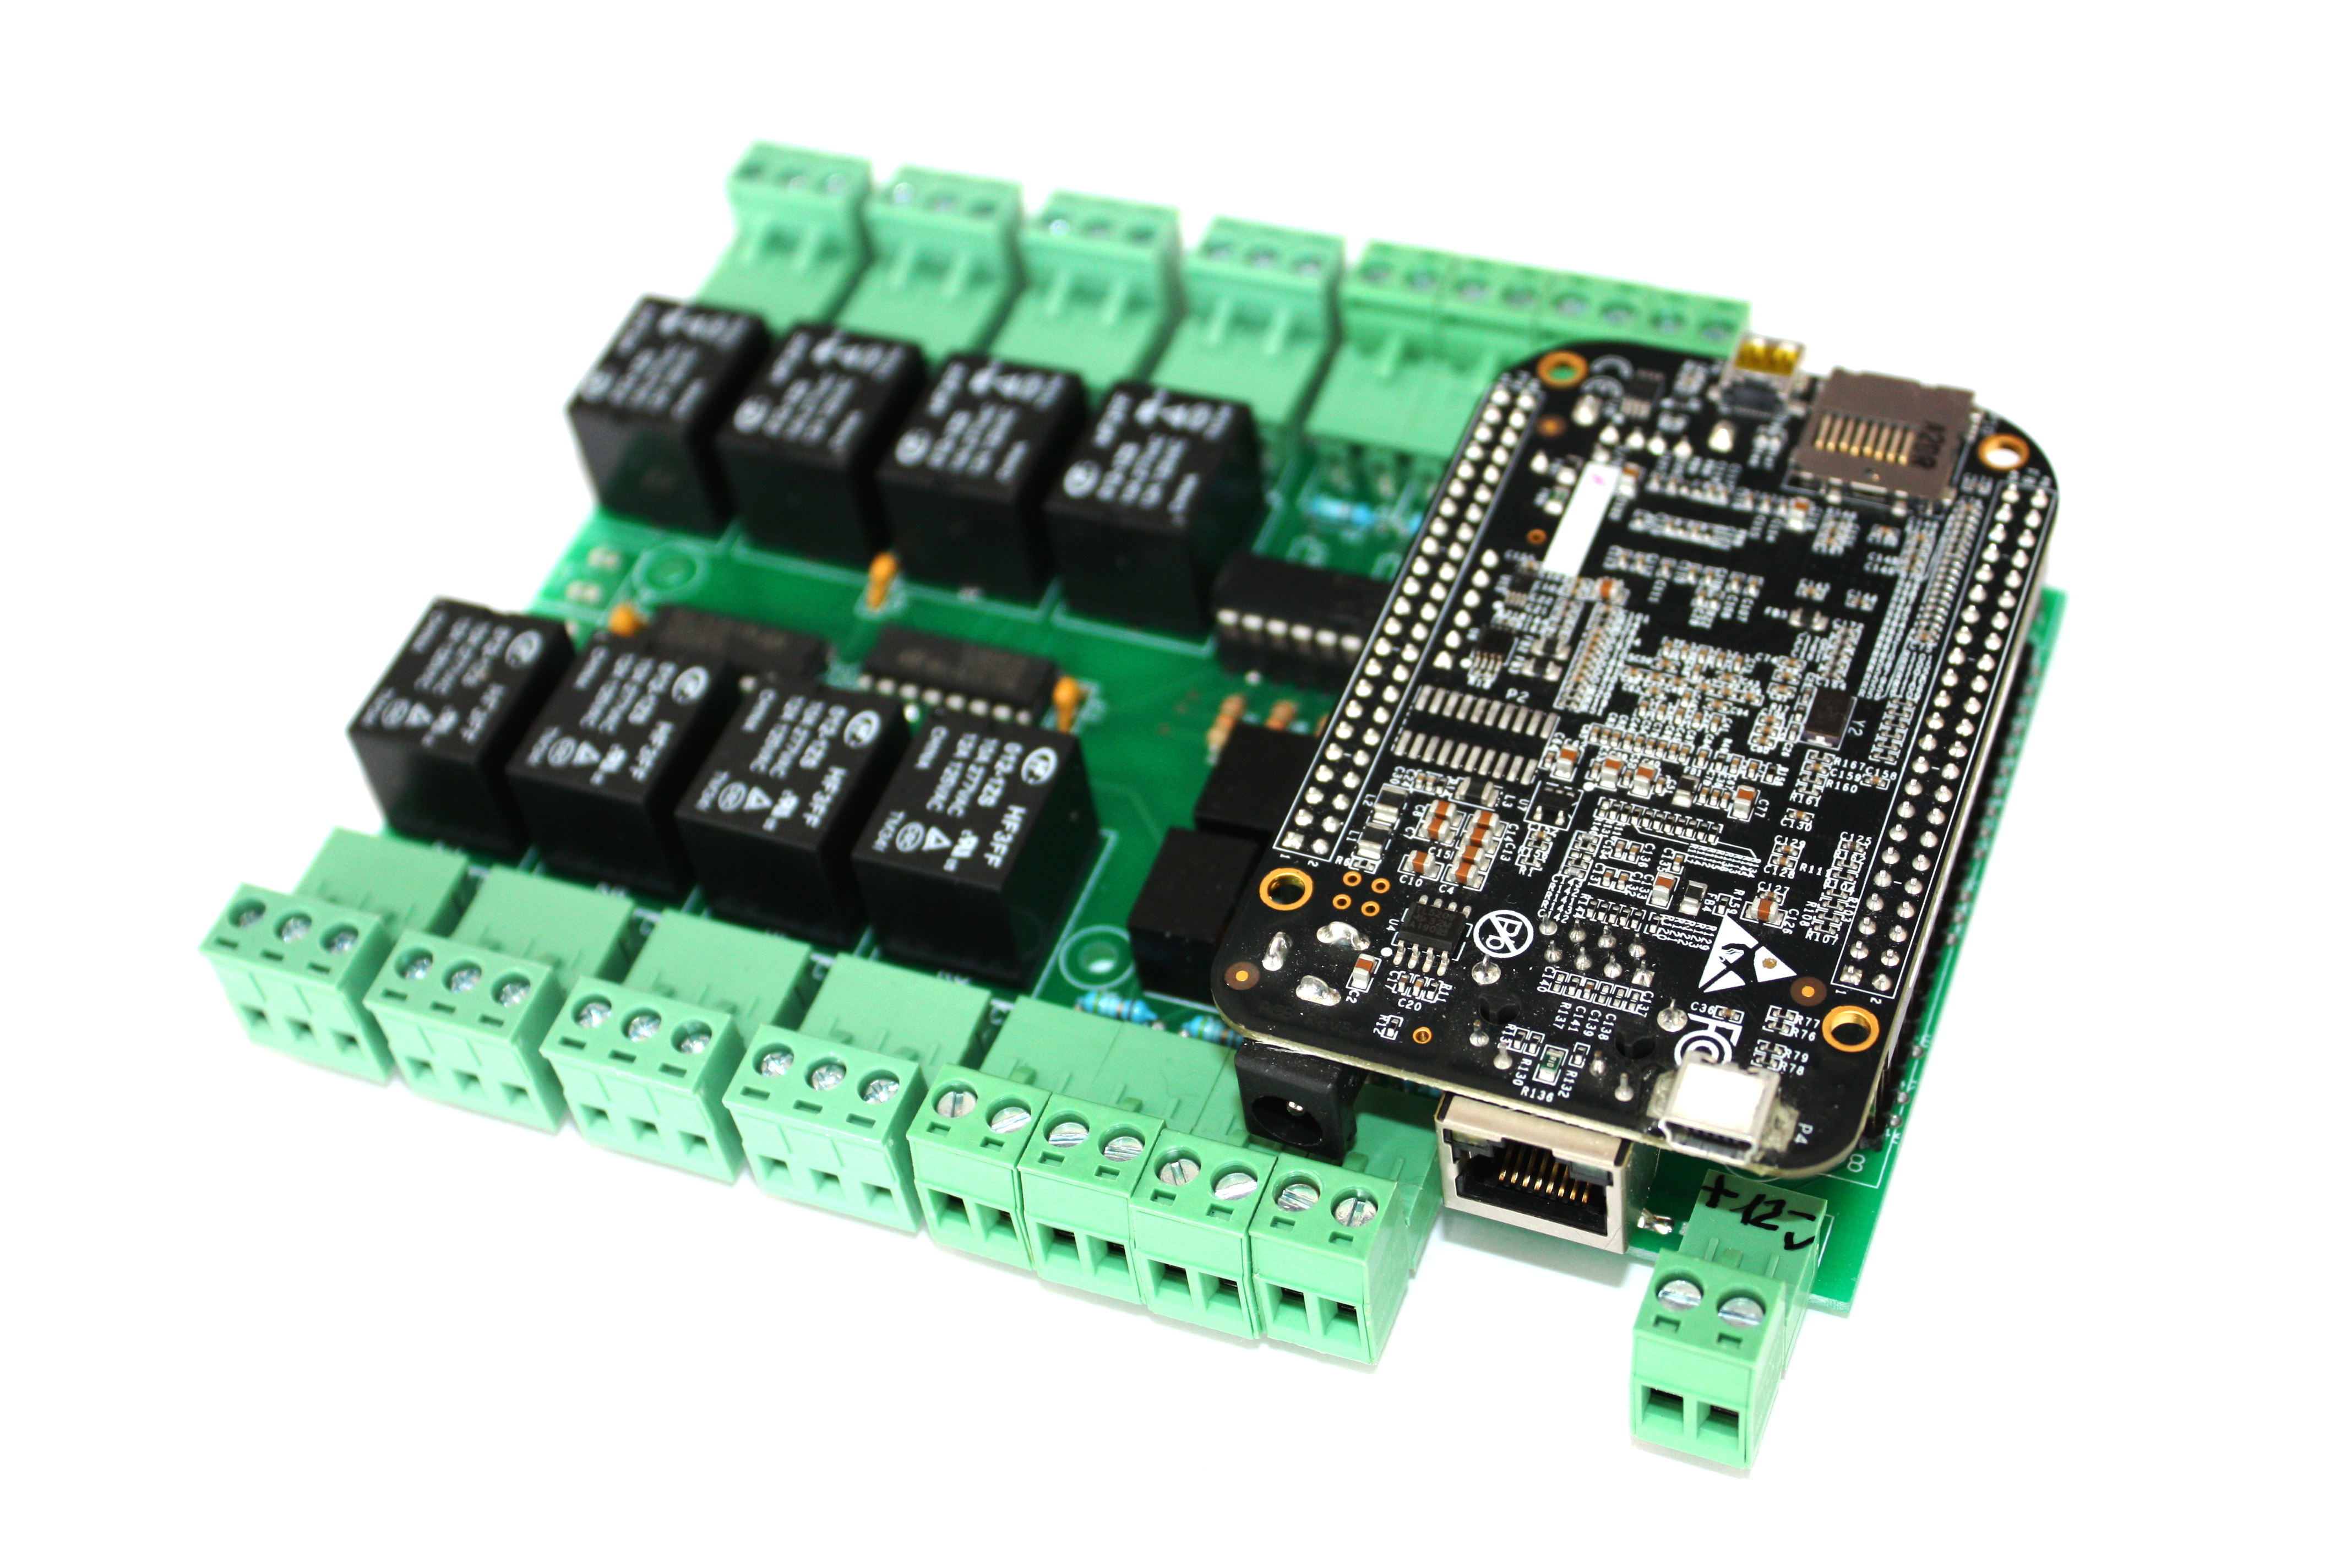
\includegraphics[width=\textwidth,natwidth=585,natheight=180]{assets/images/beaglebone.jpg}
                \caption{BeagleBone Black e OSSO Cape}
                \label{fig:bbb}
        \end{center}
\end{figure}

Essa placa traz o conceito de \textit{capes}, que nada mais são que placas não-oficiais que permitem expandir uso das saídas e entradas da BeagleBone. Nesse projeto, foi utilizada a OSSO Cape, sendo que os seguintes recursos facilitaram a implementação do protótipo:

\begin{itemize}
  \item Oito entradas digitais optoacopladas
  \item Oito saídas digitais por meio de relês
  \item Saída RS-485 integrada
  \item Gerenciamento de fontes externas com tensões entre 5 à 24V
\end{itemize}

\subsection{Medidor de Energia Mult-K}
\subsection{Phoenix Controller}
\subsection{HMI WEG}

\section{Projeto de Software}

\subsection{Comunicação MODBUS entre periférios}
\subsection{Comunicação OCPP}
\subsection{Modificações Linux}
\subsection{Funcionamento do Software}

\section{Testes}

\subsection{Ferramentas de teste}
\subsection{Testes iniciais}
\subsection{Testes na estação protótipo}

\section{Ferrame}
